\documentclass[runningheads]{llncs}

% --- Springer's official LNCS preamble (samplepaper.tex, llncs.cls v2.25) ---
\usepackage[T1]{fontenc}
\usepackage{newtxtext}
\usepackage[varvw]{newtxmath}
\usepackage{graphicx}

% --- Added for this paper; none of these alter the Springer layout ---
\usepackage{booktabs}
\usepackage{amsmath}
\usepackage{microtype}
\usepackage[hidelinks]{hyperref}
\usepackage{xcolor}

% Drafting helper: \todo{...} marks what is still missing.
% Comment the first line and uncomment the second before submitting.
\newcommand{\todo}[1]{\textcolor{red}{[TODO: #1]}}
%\newcommand{\todo}[1]{}

\begin{document}

\title{Lessons from the SIMBig 2026 Shared Task on Puno Quechua ASR}

% Runs in the page header; llncs requires it when the title is long.
\titlerunning{Puno Quechua ASR at SIMBig 2026}

\author{Raymond Negron \and Rosa Y. G. Paccotacya-Yanque}
\authorrunning{R. Negron and R. Y. G. Paccotacya-Yanque}

\institute{Department of Computing, Universidad Cat\'olica San Pablo,
Arequipa, Peru\\
\email{\{raymond.negron,rypaccotacya\}@ucsp.edu.pe}}

\maketitle

\begin{abstract}
We describe our system for Task~1 of the SIMBig~2026 shared task on automatic
speech recognition for Puno Quechua (ISO 639-3: \texttt{qxp}). We fine-tune the
published XLS-R-300M checkpoint, already adapted by continued pre-training, for
500 updates on the organisers' curated reference text, and decode spontaneous
speech with a character $n$-gram language model under lexicon-free beam search.
Relative to the published baseline, mean word error rate falls from 13.15 to
9.14 under the established speaker-disjoint split, a gain that comes mostly
from the curated orthography rather than from acoustic modelling. Because that
split shares every development sentence with training, we select systems on a
speaker- and text-disjoint split and report a held-out set measured once. We
also report three approaches that did not help: averaging CTC logits across
seeds, stronger SpecAugment masking, and language-model weights tuned on
development data.

\keywords{Automatic speech recognition \and Low-resource languages \and
Quechua \and Evaluation methodology \and Self-supervised learning.}
\end{abstract}

\section{Introduction}
\label{sec:intro}

Puno Quechua (ISO 639-3: \texttt{qxp}) belongs to the Southern Quechua branch
and is spoken by approximately 465{,}000 people in the Puno region of
Peru~\cite{huaman2026punoasr}. Formal education in the region is conducted
almost entirely in Spanish, so most speakers are fluent in Quechua but cannot
read or write it. That asymmetry is what makes speech recognition the
appropriate technology here rather than a convenience: a text interface excludes
precisely the people the technology is meant to serve, while a speech interface
meets them where their literacy already is.

Speech resources for Quechua exist for other varieties
\cite{cardenas2018siminchik,paccotacya2022collao}, but until recently none was
dedicated to this one. Huaman et
al.~\cite{huaman2026punoasr} released the first through a participatory
campaign: 66 hours of recordings, a benchmark across four architectures, and
open checkpoints. We start from their best system and take part in Task~1 of
the SIMBig~2026 shared task, which evaluates Puno Quechua recognition on
held-out audio in two domains, scripted and spontaneous speech.

The task ranks systems by a mean rank over \emph{four} numbers: word and
character error rate in each of the two domains. This is not a detail of
scoring. The baseline paper reports two configurations of the same model, and
averaging the four numbers separates them sharply. The first reaches 1.19 WER
on scripted speech but 13.6 WER on spontaneous speech: excellent in one domain,
unusable in the other. The second reaches 2.11 and 3.15 on those same two
measures, giving up a little scripted accuracy for a great deal of spontaneous
accuracy. The mean ranks the second above the first, and it is the
configuration we start from. Throughout this paper we therefore report all
four numbers and their mean, and we treat an improvement that moves one of them
in the wrong direction as no improvement at all.

This paper makes three contributions:

\begin{enumerate}
  \item A system that improves the published baseline from 13.15 to 9.14 mean
        WER measured on the same split with the same reference text
        (Section~\ref{sec:results}).
  \item The first quantification of sentence overlap in the established
        evaluation split for this variety: hearing a sentence read by other
        speakers is worth 1.1 WER points, a 21\% relative reduction
        (Section~\ref{sec:overlap}).
  \item Three reproducible negative results on ensembling, regularisation and
        language model decoding (Section~\ref{sec:negative}).
\end{enumerate}

% =====================================================================

\section{Data and Experimental Protocol}
\label{sec:data}

\subsection{Corpora}

The task uses two Common Voice \cite{ardila2020commonvoice} releases for Puno
Quechua \cite{huaman2026quechua}. \emph{Scripted Speech 27.0} holds 22{,}727 validated clips, 30.49 hours from 77
speakers, drawn from only 2{,}067 distinct sentences -- so each sentence is read
by roughly eleven different people.

\emph{Spontaneous Speech 5.0} holds 7{,}305 clips, 35.41 hours from 110
speakers, recorded as free answers to 150 questions. Only 1{,}222 clips carry a human transcription, 5.81 hours; the remaining
6{,}083 have none, because transcription requires a Quechua literacy few
speakers have. The baseline
release supplies automatic ``silver'' transcriptions for these, generated with
omniASR \cite{keren2025omnilingual}, and we reuse 5{,}782 of them, adding about 21 hours of otherwise unusable speech.

\subsection{The curated reference}
\label{sec:curated}

Written Puno Quechua has no standardised orthography, and contributors spelled
as they saw fit. Scoring against that uneven text would reward reproducing
their inconsistencies rather than hearing well, so the organisers released a
curated reference for the 2{,}067 scripted sentences, and it is what the shared
task scores against. The curation is substantial: 629 sentences differ in spelling beyond case and punctuation,
adopting Puno forms --
\texttt{allqu}$\rightarrow$\texttt{alqu},
\texttt{iskay}$\rightarrow$\texttt{ishkay},
\texttt{misk'i}$\rightarrow$\texttt{mishk'i}. Each is a single-letter change,
and each costs a whole word under WER.

The published baseline predates the curated release and was trained on the raw
text, which isolates the effect exactly. We transcribed our scripted
development set once with that model and scored the resulting transcriptions,
unchanged, against each reference in turn. The model is identical in both
measurements, so any difference between them is orthography and not acoustics.
Those transcriptions score
8.13 WER and 2.76 CER against the raw reference, and 16.08 and 3.77 against the
curated one. Nearly eight points of word error rate are orthography rather than
acoustics. We therefore fine-tune on the curated reference rather than on the
raw Common Voice text (Section~\ref{sec:system}).

\subsection{Text normalisation}

The curated scripted text uses 27 symbols; the spontaneous transcriptions are
not uniform, with 243 rows carrying 28 characters outside that convention --
digits, braces, brackets, Spanish accents, three Unicode spellings of the
apostrophe and one control character. The apostrophe matters most: in Puno
Quechua it forms part of the letter for ejective consonants (\texttt{k'},
\texttt{p'}, \texttt{ch'}), so three spellings split one phoneme across three
output symbols.

We fold everything to the curated convention: lowercase, Unicode NFC,
\texttt{a}--\texttt{z}, \texttt{ñ} and the apostrophe. Two choices were
verified against the curated reference rather than assumed -- it contains no
accented vowels and no hyphens in 2{,}067 sentences -- leaving a 29-symbol
training alphabet, every symbol of which the baseline checkpoint can already
emit: its CTC layer has 50 outputs, and our 29 are a subset of them.

The folding is orthographic, not lexical: the organisers' curation also
replaces whole word forms (\texttt{allqu}$\rightarrow$\texttt{alqu}), and we
do not propagate those to the spontaneous transcriptions, which nobody curated.
The 372 substitutions recoverable from the scripted diff would touch 1.20\% of
spontaneous training tokens; we leave this untested.

\subsection{Splits}
\label{sec:splits}

The baseline's split, which we reproduce as \texttt{sharedtask}, assigns whole
speakers to each partition, balancing gender and duration. It separates
speakers cleanly but cannot separate text: the training portion holds all
2{,}067 sentences, so every development sentence appears there, read by other
people. On the baseline's own released split, 805 of 805 development sentences
and 757 of 757 test sentences also occur in training.

We therefore built a second split, \texttt{sharedtask\_both}, disjoint in
speakers \emph{and} text. Holding out sentences costs clips, so its development
portion falls to 339 scripted clips against 1{,}493; with 1{,}347 reference
words, one WER point is thirteen words, and we treat differences below a few
tenths as noise throughout.

We use both, as Figure~\ref{fig:pipeline} summarises: decisions are made on
\texttt{sharedtask\_both}, where no development sentence has been heard in
training, while
the comparison against the published baseline is reported on
\texttt{sharedtask}, the ruler the baseline was measured with.
The spontaneous side needs no reconstruction -- its release carries an official
\texttt{split} column, which we adopt unchanged, excluding the 296 clips marked
as test from training and development alike.

\subsection{The held-out set}
\label{sec:heldout}

A development set that has driven every decision -- ours drove step counts,
learning rates, 72 language model configurations and the decoder per domain --
is no longer an unbiased estimate. None of that is training in the gradient
sense, but all of it is selection, and selection leaves a mark.

We therefore reserved a held-out portion when the splits were built, never
looked at it, and measured it once, after every decision here was frozen. To
make the commitment checkable rather than merely stated, the expected figures
were pre-registered in the evaluation script's header before it ran. Nothing
was changed afterwards.

\section{System}
\label{sec:system}

\subsection{Acoustic model}

We start from the baseline's strongest balanced checkpoint: XLS-R-300M
\cite{babu2022xlsr}, a multilingual wav2vec~2.0 model
\cite{baevski2020wav2vec2} of 315M parameters, continued pre-training on 65 hours of
unlabelled Puno Quechua audio, then CTC fine-tuning \cite{graves2006ctc} on
validated and silver data. Continued pre-training is what adapts a multilingual
model to the phonology of a language it has barely seen, and is reliably worth
its cost in low-resource settings \cite{dehaven2022cpt,getman2024adaptation};
we reuse the authors' checkpoint rather than replicate it.

The released checkpoints are fairseq files, and fairseq 0.12.2 has no wheel for
current Python versions, so we port the weights to the HuggingFace
\texttt{Wav2Vec2ForCTC} implementation \cite{wolf2020transformers}.
As a correctness check, the converted model scores 27.26 WER on the baseline's
out-of-domain set against its published 27.4, confirming the port is faithful.

Fine-tuning runs for 500 updates at learning rate $2\times10^{-5}$
(Section~\ref{sec:plateau}). Batches are formed by total audio duration rather
than clip count: clips range from under two seconds to thirty, so any fixed
count either exhausts memory on long clips or wastes the device on short ones.


\begin{figure}[tb]
\centering
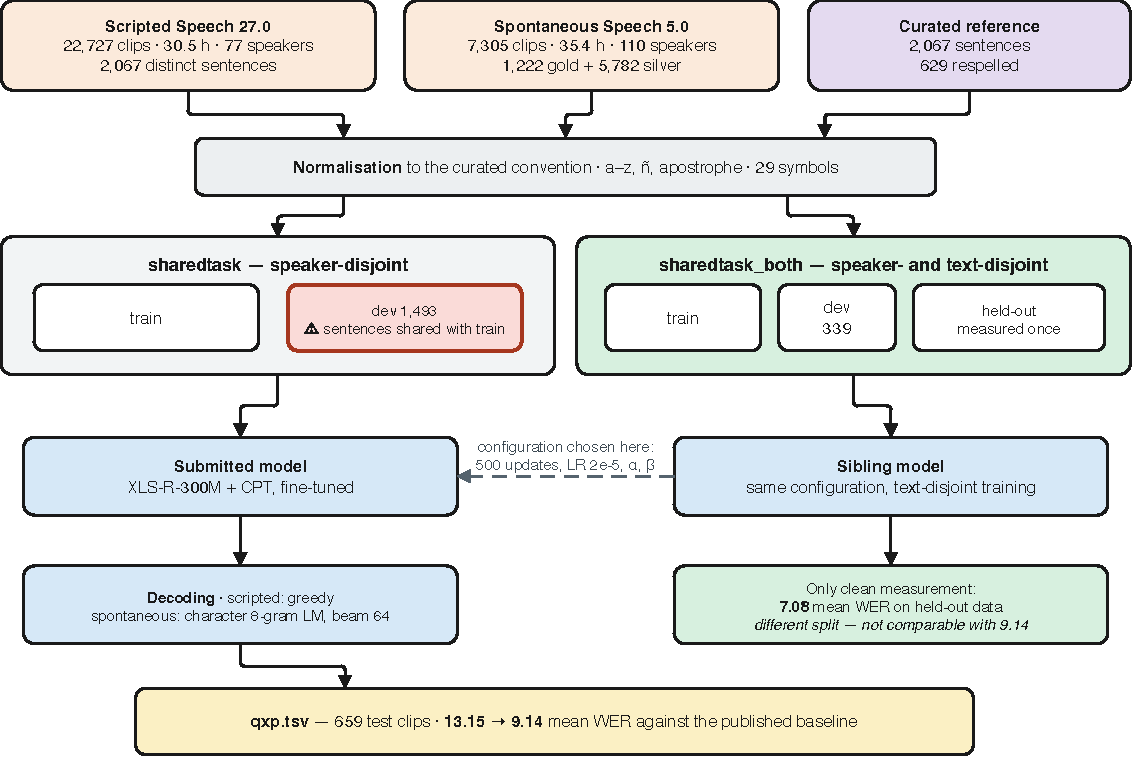
\includegraphics[width=\textwidth]{figures/pipeline_pastel.pdf}
\caption{Data, splits and system. Two splits are built from the same
normalised corpora. The submitted model trains on \texttt{sharedtask}, whose
development sentences also occur in training; its sibling trains on
\texttt{sharedtask\_both}, which shares neither speakers nor sentences and so
yields the only measurement free of overlap. The dashed arrow marks what
passes between them: the configuration is chosen on the sibling and applied to the
submitted model, not its weights.}
\label{fig:pipeline}
\end{figure}

\subsection{Decoding}

Spontaneous speech is decoded with a language model over characters rather
than words; Section~\ref{sec:discussion} explains why. These language models
are character $n$-grams estimated by counting, with modified
Kneser-Ney smoothing \cite{chen1996smoothing} to reserve probability for
sequences the training text never shows. We check each one against KenLM
\cite{heafield2011kenlm}: a distribution must sum to one, so for 200 contexts
we sum the probability of every possible next character; the largest deviation
was of order $10^{-6}$.

Decoding uses flashlight-text's \emph{lexicon-free} beam search
\cite{kahn2022flashlight} with beam width 64. The qualifier matters: a
conventional decoder consults the language model only when a word ends, against
a fixed vocabulary, which a character model cannot use. A lexicon-free decoder
scores it on every character as it is emitted. A hypothesis scores
\begin{equation}
\sum \log p_{\text{CTC}}
\;+\; \alpha \sum \log P_{\text{LM}}
\;+\; \beta\,n_{\text{words}},
\label{eq:score}
\end{equation}
where $\alpha$ weights the language model against the acoustics and $\beta$
offsets its preference for shorter word sequences.

The final configuration decodes scripted speech greedily and spontaneous speech
with an order-8 model trained on gold and silver spontaneous text,
$\alpha = 0.5$, $\beta = 0$. Section~\ref{sec:lmneg} explains why scripted
speech ends up with no language model at all.

\section{Results}
\label{sec:results}

\begin{table}[tb]
\centering\small
\caption{Main results, all figures percentages, scored against the curated
reference. The two blocks are \emph{different models} on \emph{different
splits}. Above: the system we submit, against the published baseline, both on
the established split. Below: its sibling, trained on the text-disjoint split
and therefore the only model we can measure without sentence overlap; its
held-out row was measured once, after every decision was frozen. The two
upper rows are single models, so no seed statistics apply to them.}
\label{tab:main}
\begin{tabular}{lrrrrrr}
\toprule
& \multicolumn{2}{c}{Scripted} & \multicolumn{2}{c}{Spontaneous} & \multicolumn{2}{c}{Mean} \\
\cmidrule(lr){2-3}\cmidrule(lr){4-5}\cmidrule(lr){6-7}
System & WER & CER & WER & CER & WER & CER \\
\midrule
\multicolumn{7}{l}{\emph{Submitted model, on \texttt{sharedtask} development (speaker-disjoint)}} \\
\quad Published baseline, converted & 16.08 & 3.77 & 10.23 & 1.39 & 13.15 & 2.58 \\
\quad This work & 9.23 & 3.01 & 9.06 & 1.30 & \textbf{9.14} & 2.16 \\
\addlinespace
\multicolumn{7}{l}{\emph{Sibling model, trained and measured on \texttt{sharedtask\_both}}} \\
\multicolumn{7}{l}{\emph{(speaker- and text-disjoint), mean of three seeds}} \\
\quad on its development set & 4.85 & 0.62 & 9.20 & 1.31 & 7.02 & 0.96 \\
\quad\quad \emph{std.\ dev.\ across seeds} & 0.21 & 0.04 & 0.18 & 0.02 & 0.19 & 0.03 \\
\quad on its held-out set & 10.79 & 2.33 & 3.38 & 0.39 & 7.08 & 1.36 \\
\quad\quad \emph{std.\ dev.\ across seeds} & 0.14 & 0.02 & 0.07 & 0.01 & 0.05 & 0.01 \\
\bottomrule
\end{tabular}
\end{table}

\subsection{How long to train}
\label{sec:plateau}

Fine-tuning from an already-adapted checkpoint needs far less training than the
original 8{,}000 updates. On the text-disjoint split, every configuration
between 250 and 1{,}000 updates and between $1\times10^{-5}$ and
$5\times10^{-5}$ lands at 7.1--7.3 mean WER: below about 200 updates the
curated orthography is not yet learned, beyond about 1{,}000 the model
memorises, and by 8{,}000 it is worse than at 500. The useful conclusion is a
broad plateau, not an optimum.

Reaching that conclusion required a correction worth reporting. A single run at
500 updates and $2\times10^{-5}$ gave 6.96 mean WER, best of every
configuration on all four numbers, and we recorded it as the winner; a second
seed of the identical configuration gave 7.26. Three seeds measure the noise directly:
7.02 mean WER with standard deviation 0.19 on the text-disjoint development
set, and 9.23 with deviation 0.08 on the larger speaker-disjoint one, of which
Table~\ref{tab:main} reports the submitted seed. We treat any difference below
roughly 0.3 mean WER as indistinguishable from the random draw. The contrast between the two sets is easy to overlook when choosing one:
the smaller does not merely measure less precisely, it manufactures differences.

\subsection{Sentence overlap, measured}
\label{sec:overlap}

Section~\ref{sec:newsentences} makes the established split's text overlap a
measurement problem rather than a curiosity. The design holds the evaluation fixed and varies only what the model saw.
Condition~A trains on the text-disjoint split, so the development sentences
never appear. Condition~B adds the recordings of those same sentences made by
\emph{training} speakers, 3.65 hours more audio. Comparing A with B alone would
confound exposure with data volume, so condition~B$_{\text{eq}}$ removes 3.64
hours of randomly chosen A clips, leaving exactly A's 39.94 hours. Every
condition uses the same configuration, 250 updates, and the same development set.


\begin{table}[tb]
\centering\small
\caption{What hearing a development sentence from other speakers is worth.
Same development set and same configuration (250 updates) throughout; only the
training data differs. Two seeds where two figures are given.}
\label{tab:overlap}
\begin{tabular}{llrr}
\toprule
Training set & Dev sentences heard? & Scripted WER & Scripted CER \\
\midrule
A \quad (39.94 h) & no & 5.20 / 4.97 & 0.65 / 0.62 \\
B$_{\text{eq}}$ (39.94 h) & yes, same hours as A & \textbf{3.79 / 4.23} & \textbf{0.48 / 0.55} \\
B \quad (43.58 h) & yes, with 3.65 h more audio & 4.68 & 0.60 \\
\bottomrule
\end{tabular}
\end{table}

The seed ranges of A and B$_{\text{eq}}$ do not overlap -- the worse
B$_{\text{eq}}$ run still beats the better A run -- so at equal training
volume, having heard a sentence read by other speakers is worth 1.1 WER points,
a 21\% relative reduction, and about 19\% of CER.

It is a lower bound: memorisation grows with training, and the original
baseline runs for 8{,}000 updates.

\subsection{Held-out evaluation}
\label{sec:heldout-results}


The lower block of Table~\ref{tab:main} gives the measurement. The means agree
closely, 7.02 against 7.08, which is the result we care about:
after dozens of decisions taken on the development set, the held-out estimate
did not collapse, and seed spread falls to 0.05.

The agreement hides two large opposing movements, both composition rather than
generalisation. Scripted error doubles because the held-out portion contains
one speaker who alone scores 98.67 WER over 59 clips; removing that same
speaker from the development set moves its scripted WER from 9.23 to 5.71.
Spontaneous error falls by two thirds because 46\% of the held-out spontaneous
portion comes from speakers already heard through silver transcriptions in
training. With 77 scripted speakers, a split places few voices in each
partition, so no such figure should be read without its per-speaker breakdown.

% =====================================================================

\section{Approaches Without Measurable Gains}
\label{sec:negative}

This section describes other approaches tested for the competition that did not
yield positive results.

\subsection{Averaging CTC models across seeds}

We explored an ensemble of the models across seeds, which did not improve
results. Seed noise of 0.3 mean WER is what ensembling should remove, so a gain
was the expectation; neither fusion rule delivers one. CTC emits sharp peaks at particular
frames, and independently trained models place them at adjacent but not
identical frames; averaging logits is a geometric mean, so a confident peak
averaged against a near-zero value collapses and the letter disappears.
Character deletions rise from 21 to 50 and mean WER from 7.02 to 8.38.
Averaging probabilities stops deleting letters but gains nothing, at 7.30. With
CTC's peaky, time-shifted alignments the fusion rule matters more than the
ensemble.

\subsection{Stronger SpecAugment masking}

Overfitting past 1{,}000 updates is the failure mode we observed, and
SpecAugment \cite{park2019specaugment} addresses it directly. Raising the
time-masking probability from the default 0.05 to 0.2 and 0.5 gives 6.81, 7.05
and 7.68 mean WER: monotonically worse, on all four numbers. With a 500-update
schedule there is little time to overfit, and masking removes evidence the
model has few chances to see.

\subsection{The language model stops helping on held-out data}
\label{sec:lmneg}

On scripted speech no setting gains measurably once the acoustic model is this
accurate: every configuration sits within $\pm0.15$ WER of greedy decoding,
about two words, so we decode scripted speech without a language model.

On spontaneous speech it gains on development data, by 0.31, 0.17 and 0.12 WER
across three seeds, but on held-out data the identical configuration gains 0.00
and loses 0.04 and 0.08. We keep it, since the held-out effect is within noise
either way, but no longer claim it helps.

An earlier version of this tuning shows the hazard more sharply. Run on the
speaker-disjoint development set, the grid selects $\alpha = 2.0$ and reports
4.54 scripted WER, because at that weight the language model recalls whole
development sentences it was built from; under the new-sentence condition the
same setting yields 9.83, worse than greedy.

% =====================================================================

\section{Discussion}
\label{sec:discussion}

Read-speech corpora for low-resource languages are built the way this one was:
a small pool of sentences recorded many times over by the few speakers who
volunteer -- here 2{,}067 sentences and 77 speakers. Any split that separates speakers while using all the recordings therefore
evaluates with complete text overlap, by construction rather than oversight:
the training portion must contain every sentence to contain every clip. We report this as a
property of the benchmark, and it is consequential: a development set whose
sentences the model has already heard from other speakers prefers systems that
remember text over systems that recognise speech.

The remedy is cheap: report the text-disjoint figure alongside the conventional
one. Where a corpus ships an official split disjoint in both respects, as
Common Voice does here at the cost of one recording per sentence, the lost
training data buys one honest measurement among the optimistic ones.

Decoding is the other place where the shape of the data decides the method.
Greedy CTC decoding commits to the most probable symbol at each 20\,ms frame
independently, with no notion of the word being formed, and the error profile
shows what that costs: on the baseline's out-of-domain set we measure 23.4\%
substitutions against almost no deletions or insertions -- the signature of
words that are nearly right. That invites a language model, and it must be over
characters: Quechua builds words by chaining suffixes, and 77\% of the distinct
word forms in the scripted sentence corpus occur exactly once, so a word-level
model would never have seen the correct form of most words it must judge.

% =====================================================================

\section{Limitations}
\label{sec:limitations}

\textbf{The submitted system's development figures are affected by
sentence-level leakage.} It is trained on the established split, whose training
portion contains every development sentence, read by other speakers; no
development audio and no official test audio were used in training. Its
development scores are therefore optimistic. We submit it for comparability
with the published baseline and because it sees 15\% more distinct sentences
than the text-disjoint model.

\textbf{The search was narrow:} we varied updates and learning rate only.
Batch size, spontaneous upsampling, layer dropout, accent folding and the
inclusion of silver data were left at their defaults.

\textbf{Three seeds} are enough to establish that several apparent wins were
noise, too few to separate configurations differing by less than their spread.

\textbf{Half the ranking cannot be measured faithfully.} The spontaneous test
consists entirely of speakers aged sixty or over, and speakers of that age are
a small and almost unlabelled part of the corpus: 2.90 of its 35.41 hours of
spontaneous audio, some 8\%, across which exactly one clip carries a human
transcription. No development or held-out set we can construct therefore
contains gold elderly spontaneous speech, so the domain deciding half our rank
is the one we can least evaluate.

% =====================================================================

\section{Conclusion}
\label{sec:conclusion}

We fine-tuned the published XLS-R-300M checkpoint for 500 updates on the
organisers' curated reference text and decoded spontaneous speech with a
character $n$-gram model, improving the published baseline from 13.15 to 9.14
mean WER on the same split with the same reference. Most of that gain is
orthography rather than acoustics.

The methodological result may outlast the system: the established split shares
every evaluation sentence with training, worth 1.1 WER points, while the shared
task's own test does not. Three things we expected to help did not. Gold transcriptions from elderly
speakers would make half of this benchmark measurable for the first time.


% llncs v2.25 expects acknowledgements and declarations inside `credits`.
\begin{credits}
\subsubsection{\ackname}
This work was developed using the computational infrastructure of Project
No.~\todo{number} funded by ProCiencia.

\subsubsection{\discintname}
The authors have no competing interests to declare that are relevant to the
content of this article.
\end{credits}

\subsubsection{Resources.} Code, splits and configurations are available at
\url{https://github.com/raymond1242/asr-puno-quechua}.

\bibliographystyle{splncs04}
\bibliography{refs}

\end{document}
